\problemset{Статистический анализ}
\problemset{Индивидуальное домашнее задание №2}

\renewcommand*{\proofname}{Решение}
\textbf{Часть 1}

В результате эксперимента получены данные. \\

\begin{tabular}{|c|c|c|c|c|c|c|c|c|c|c|c|c|c|c|c|c|c|c|c|c|c|c|c|c|}
	\hline
	3&3&3&5&4&2&0&4&4&1&2&3&1&2&1&3&3&2&4&3&5&4&2&3&3\\ \hline 1&4&3&2&4&6&3&3&4&4&7&1&3&1&1&1&3&3&2&6&5&1&3&2&6\\
	\hline 
\end{tabular}
\\


	$\alpha_1=0.01$ 
	
	$a = 1.27$ 
	
	$b = 3.69$ 
	
	$\lambda_0=4.00$ 
	
	$\lambda_1=3.00$ \\

\begin{problem}
	Построить вариационный ряд, эмпирическую функцию распределения и гистограмму частот.
\end{problem}

\begin{proof}
	$ $
		
	Вариационный ряд:
	
	0 1 1 1 1 1 1 1 1 1 2 2 2 2 2 2 2 2 3 3 3 3 3 3 3 3 3 3 3 3 3 3 3 3 4 4 4 4 4 4 4 4 4 5 5 5 6 6 6 7 
	
	Построим таблицу частот для выборки.
	\begin{table}[h]
    \centering	
	\begin{tabular}{|c|c|c|c|c|c|c|c|c|}
		\hline
		$x_j$&0&1&2&3&4&5&6&7\\ \hline
		$m_j$&1&9&8&16&9&3&3&1\\ \hline
		$p_j^*$&0.02&0.18&0.16&0.32&0.18&0.06&0.06&0.02\\
		\hline
	\end{tabular}
	\end{table}
	
	Построим эмпирическую функцию распределения по полученным данным:\\
	
	 $F(x)=\left\{ 
	\begin{gathered} 
		0, x \leqslant 0 \hfill \\  
		0.02, 0 < x \leqslant 1 \hfill \\
		0.20, 1 < x \leqslant 2 \hfill \\
		0.36, 2 < x \leqslant 3 \hfill \\
		0.68, 3 < x \leqslant 4 \hfill \\
		0.86, 4 < x \leqslant 5 \hfill \\
		0.92, 5 < x \leqslant 6 \hfill \\
		0.98, 6 < x \leqslant 7 \hfill \\
		1, x > 7 \hfill \\
	\end{gathered}
	\right.$	
	\begin{figure}[h]
		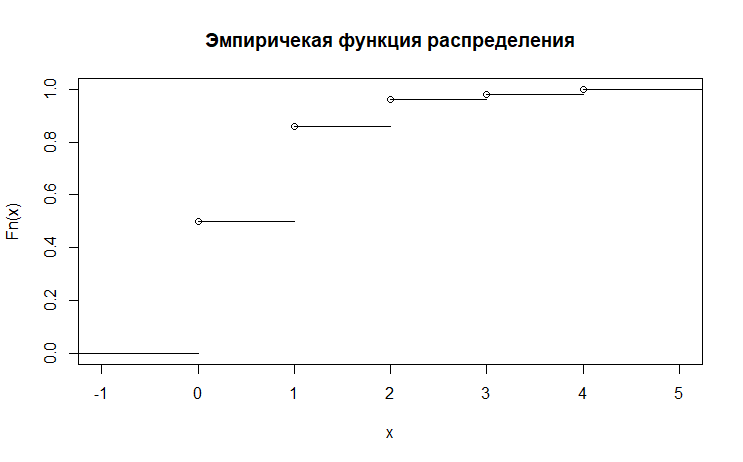
\includegraphics[scale=0.85]{Emp.png}
	\end{figure}
	\begin{figure}[h]
		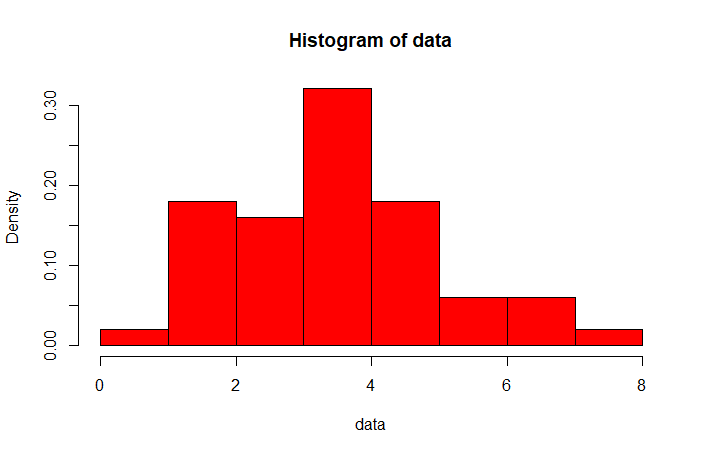
\includegraphics[scale=0.85]{Hist.png}
	\end{figure}
\end{proof}
\newpage

\begin{problem}
	Вычислить выборочные аналоги характеристик:
\end{problem}

\begin{proof}
	$ $
	
	\begin{enumerate}
	\item Математическое ожидание:
		\begin{equation}	
		\bar x_{\text{в}} = \cfrac1n\sum^{n}_{i=1}x_i m_i=2.98
		\end{equation}
	\item Дисперсия:
	\begin{equation}	
		D_{\text{в}} = \bar{x^2}-\bar{x}^2=\cfrac1n\sum(x_i-\bar{x})^2=2.3396
	\end{equation}
	\item Медиана:
	\begin{equation}
		Me = 3
	\end{equation}	
	\item Ассиметрия:
	\begin{equation}
		As = \cfrac{\mu_3^*}{\sigma^3} = 0.4230174
	\end{equation}
	\item Эксцесс:
	\begin{equation}
		Ex = \cfrac{\mu_4^*}{\sigma^4}-3 = -0.09535895
	\end{equation}
	\item Вероятность:
	\begin{equation}
		P(x \in [a, b]) = P(x \in [1.27, 3.69]) = F(3.69) - F(1.27) = 0.48 
	\end{equation}
	\end{enumerate}			
\end{proof}


\begin{problem}
	В предположении, что исходные наблюдения являются выборкой из распределения Пуассона, построить оценку максимального правдоподобия параметра $\lambda$, а также оценку $\lambda$ по методу моментов. Найти смещение оценок 	
\end{problem}

\begin{proof}
	$ $ 
	
	Распределение Пуассона:
	$P_{\lambda} = (x = k) = \cfrac{\lambda^k}{k!}\cdot \exp(-\lambda)$
	\begin{enumerate}
		\item Метод максимального правдоподобия \\
			$l(x, \lambda) =  \cfrac{\lambda^{\sum\limits^n_1x_i}\cdot \exp (-\lambda n)}{\prod\limits_1^n x_i!}\Rightarrow$ 
			$ll(\bar{x}, \lambda) =\sum\limits_1^nx_iln\lambda-n\lambda-\sum\limits_1^nlnx_i!\Rightarrow$ \\ $\cfrac{\partial ll(\bar x, \lambda)}{\partial \lambda} = \cfrac1{\lambda}\sum\limits_1^nx_i-n=0\Rightarrow \hat{\lambda}= \cfrac{1}{n}\sum\limits_1^nx_i=\bar{x_{\text{в}}}=2.98$ \\
		\item Метод моментов \\
			$P(x, \theta)$ \\
			$M_1^* = \bar{x_{\text{в}}}; \mathbb{E}X = \bar{x_{\text{в}}};$ \\
			$\mathbb{E}X = \int_{\mathbb{R}}xp(x, \theta)dx = \varphi(\theta)$ \\
			$M_1 = \mathbb{E}X=\lambda; M_1^* = \bar{x_{\text{в}}} \Rightarrow \hat{\lambda} = \bar{x_{\text{в}}} = 2.98$
	\end{enumerate}
	Чтобы найти смещение оценки, найдем: \\
		$\mathbb{E}\hat{\lambda}=\cfrac1n\sum\limits_1^n\mathbb{E}x_i=\cfrac{n\lambda}n=\lambda\Rightarrow\text{оценки несмещенные}$
\end{proof}


\begin{problem}
	Построить асимптотический доверительный интервал уровня значимости $\alpha_1$ для параметра $\lambda$ на базе оценки максимального правдоподобия.	
\end{problem}

\begin{proof}
        $ $

		$\hat{\lambda}=\bar{x_{\text{в}}}=2.98; \alpha_1=0.01; \gamma=1-\alpha_1=0.99;$ \\
		$\cfrac{\sqrt{n}(\bar{x}-\lambda)}{\sqrt{\lambda}}\underset{n\to\infty}{\longrightarrow}N(0,1)$ \\
		$t_\gamma: \phi(t_\gamma)=1-\cfrac{\alpha_1}2\Rightarrow t_\gamma=2.575829$ \\
		$P(-t_\gamma \leqslant \cfrac{\sqrt{n}(\bar{x_\text{в}}-\lambda)}{\sqrt{\lambda}} \leqslant t_\gamma)\longrightarrow 1-\alpha$ \\
	    $n(\bar{x_\text{в}}-\lambda)^2=t_\gamma^2\lambda$ \\
		$\lambda^2-2\lambda(\bar{x_\text{в}}+\cfrac{t_\gamma^2}{2n})+\bar{x_\text{в}}=0$ \\
	$\lambda_{1,2}=\bar{x_\text{в}}+\cfrac{t_\gamma^2}{2n}\pm t_\gamma\sqrt{\cfrac1n(\bar{x_\text{в}}+\cfrac{t_\gamma^2}{4n})}\Rightarrow [2.35116; 3.60884]$ 
\end{proof}


\begin{problem}
	Используя гистограмму частот, построить критерий значимости $\chi^2$ проверки простой гипотезы согласия с распределением Пуассона с параметром $\lambda_0$. Проверить гипотезу на уровне значимости $\alpha_1$. Вычислить наибольшее значение уровня значимости, на котором еще нет оснований отвергнуть данную гипотезу. 
\end{problem}

\begin{proof}
		$\hat{\lambda_0}=4.00; \alpha_1=0.01;$ \\
		$\text{Простая гипотеза } H_0 \text{ имеет вид:}$ \\
		$H_0:p(x)=\cfrac{\lambda_0^x}{x!}\exp(-\lambda_0)$ \\
		$p_k=P(X=k)=\cfrac{0.7^k}{k!}\exp(-0.7)$ \\
	Построим таблицу оценки методом $\chi^2$. \\
	
	\begin{tabular}{|c|c|c|c|c|c|c|c|c|c|}
		\hline
		$x_i$ & $0$ & $1$ & $2$ & $3$ & $4$ & $5$ & $6$ & $7$ & $\sum$ \\ \hline 
		$m_i$ & $1$ & $9$ & $8$ & $16$ & $9$ & $3$ & $3$ & $1$ & $50$ \\ \hline 
		$p_i$ & $0.018$ & $0.073$ & $0.147$ & $0.195$ & $0.195$ & $0.156$ & $0.104$ & $0.111$ & $1$ \\ \hline 
		$m_i^{'}$ & $0.916$ & $3.663$ & $7.326$ & $9.768$ & $9.768$ & $7.815$ & $5.210$ & $5.534$ & $50$ \\ \hline 
		$m_i-m_i^{'}$ & $0.084$ & $5.337$ & $0.674$ & $6.232$ & $-0.768$ & $-4.815$ & $-2.210$ & $-4.534$ & $0$ \\ \hline 
		$\cfrac{(m_i-m_i^{'})^2}{m_i^{'}}$ & $0.008$ & $7.775$ & $0.062$ & $3.975$ & $0.060$ & $2.966$ & $0.937$ & $3.714$ & $\chi^2_{\text{набл}}$ \\
		\hline
	\end{tabular} 

	\begin{align}
		&\chi^2_{\text{набл}}=\sum\limits_1^k\cfrac{(m_i-m_i^{'})^2}{m_i^{'}}=19.49903 \\ 
		&l=k-r-1=8-1-1=6 \\
		&\chi^2_{\text{кр}}=\chi^2_{\alpha;l} = \chi^2_6  = 16.81189 \\
	\end{align}
	$\chi^2_{\text{набл}} > \chi^2_{\text{кр}}\Rightarrow$ гипотеза $H_0$ отвергается.\\
	Наибольшее значение уровня значимости, при котором еще нет оснований отвернуть данную гипотезу = $0.003398824$	
\end{proof}


\begin{problem}
	Построить критерий значимости $\chi^2$ проверки сложной гипотезы согласия с распределением Пуассона. Проверить гипотезу на уровне значимости $\alpha_1$. Вычислить наибольшее значение уровня значимости, на котором еще нет оснований отвергнуть данную гипотезу. 
\end{problem}

\begin{proof}
	$ $
	
	Сложная гипотеза $H_0$ имеет вид:
	\begin{align}
		H_0: x_1,...,x_n \sim P_{ois}(\lambda) \\
		\sum\limits_1^k\cfrac{(m_i-np_i(\lambda))^2}{np_i(\lambda)}\longrightarrow\chi^2_{k-r-1}
	\end{align}	

	Метод минимизации хи-квадрат:
	\begin{equation}
		\underset{\lambda}{argmin}\sum\limits_1^r\cfrac{(m_i-np_i(\lambda))^2}{np_i(\lambda)}
	\end{equation}
	
	Задача реализована в R следующим скриптом: 
	
	$\begin{gathered}
		P <- function(a)\{ \hfill \\
        p <- 0 \hfill \\
        p[1] <- ppois(0, a) \hfill \\
        p[2] <- ppois(1, a) - sum(p) \hfill \\
        p[3] <- ppois(2, a) - sum(p) \hfill \\
        p[4] <- ppois(3, a) - sum(p) \hfill \\
        p[5] <- ppois(4, a) - sum(p) \hfill \\
        p[6] <- ppois(5, a) - sum(p) \hfill \\
        p[7] <- ppois(6, a) - sum(p) \hfill \\
        p[8] <- 1-sum(p) \hfill \\
        p\}; X2 <- function(a)\{g <- n*P(a); f <- (nu-g)^2/g; sum(f)\} \hfill \\
        nu <- c(1,9,8,16,9,3,3,1); XM <- nlm(X2, lambda0) \hfill \\
	\end{gathered}$ \\
	
	В результате вычислений получим, что $\chi^2_{\text{набл}}=5.400952<\chi^2_{\text{крит}}=15.08627$ 
	Таким образом, гипотеза принимается. 
	
	Наибольшее значение уровня значимости, при котором еще нет оснований отвернуть данную гипотезу = $0.3689291$	
\end{proof}

\begin{problem}
	Построить наиболее мощный критерий проверки простой гипотезы пуассоновости с параметром $\lambda=\lambda_0=4.00$ при альтернативе пуассоновости с параметром $\lambda=\lambda_1=3.00$. Проверить гипотезу на уровне значимости $\alpha_1$. Что получится, если поменять местами основную и альтернативную гипотезы?
\end{problem}

\begin{proof}
	$ $
	
	Сформулируем гипотезы. 
	
	$H_0:\lambda=\lambda_0=4.00$ 
	
	$H_1:\lambda=\lambda_1=3.00$ 
	
	По лемме Неймана-Пирсона: \\
		
	$\phi(\bar x)=\left\{
	\begin{gathered}
		0, \text{if } l(\bar x, \lambda_0, \lambda_1)<C \hfill \\
		p, \text{if } l(\bar x, \lambda_0, \lambda_1)=C \hfill \\
		1, \text{if } l(\bar x, \lambda_0, \lambda_1)>C \hfill \\ 
	\end{gathered}
	\right.$
	
		$l(\bar x, 4, 3)=\cfrac{L(\bar x, 3)}{L(\bar x, 4)}=0.75^{\sum x_i}\cdot \exp(n*(\lambda_0-\lambda_1))=0.75^{\sum x_i}\cdot \exp(n)$ 
		
		$ll(\bar x, \lambda_0, \lambda_1)=\sum x_i\cdot ln0.75+n<lnC; \sum x_i < \cfrac{lnC-n}{ln0.75}; \hat{C}=\cfrac{-lnC-n}{ln0.75}$ \\
		
	Критерий принимает вид: \\
	
	$\phi(\bar x)=\left\{
	\begin{gathered}
		0, \text{if } \sum x_i<\hat{C} \hfill \\
		p, \text{if } \sum x_i=\hat{C} \hfill \\
		1, \text{if } \sum x_i>\hat{C} \hfill \\ 
	\end{gathered}
	\right.$	\\
	
	Вычислим $\hat{C}$, $p$ и $\alpha_0$:		

		$P_{\lambda_0}(l(\bar x, \lambda_0, \lambda_1)>C)+p\cdot P_{\lambda_0}(l(\bar x, \lambda_0, \lambda_1)=C)=$ 
		
		$= P_{\lambda_0}(\sum\limits_1^nx_i>\hat{C})+p\cdot P_{\lambda_0}(\sum\limits_1^nx_i=\hat{C})=\alpha_1=0.01$ 
		
		$x_i \rightarrow P_{ois}(\lambda_0); \sum x_i \rightarrow P_{ois}(n\lambda_0)$ 
		
		$\alpha_0=P_{\lambda_0}(\sum\limits_1^nx_i>\hat{C})=1-P_{n\lambda_0}(\hat{C})-p_{n\lambda_0}(\hat{C})<\alpha_1$
		
		$p=\cfrac{\alpha_1-\alpha_0}{P_{\lambda_0}(\sum\limits_1^nx_i=A)}=\cfrac{\alpha_1-\alpha_0}{p_{n\lambda_0}(A)}$ \\
	
	В результате расчета получим: $\alpha_0=0.009888703$; $\hat{C}=232$; $p=0.04845126$ 
	
		$\sum\limits_1^nx_i=149$
		
		$149<232\Rightarrow\text{ Таким образом, отвергаем гипотезу} H_0$

	Теперь поменяем местами основную и альтернативную гипотезы.	
	
	$H_0:\lambda=\lambda_1=3.00$ 
	
	$H_1:\lambda=\lambda_0=4.00$ 
	
		$l(\bar x, 3, 4)=\cfrac{L(\bar x, 4)}{L(\bar x, 3)}=(\frac43)^{\sum x_i}\cdot \exp(n*(\lambda_1-\lambda_0))=(\frac43)^{\sum x_i}\cdot \exp(-n)$ 
		
		$ll(\bar x, \lambda_0, \lambda_1)=-\sum x_i\cdot ln(\frac43)-n<lnC; \sum x_i > \cfrac{-lnC-n}{ln(\frac43)}; \hat{C}=\cfrac{-lnC-n}{ln(\frac43)}$ \\

	Тогда критерий примет вид: \\
	
	$\phi(\bar x)=\left\{
	\begin{gathered}
		0, \text{if } \sum x_i>\hat{C} \hfill \\
		p, \text{if } \sum x_i=\hat{C} \hfill \\
		1, \text{if } \sum x_i<\hat{C} \hfill \\ 
	\end{gathered}
	\right.$	\\
	
	Вычислим $\hat{C}$ и $p$.		
	
	В результате расчета получим: $\alpha_0=0.008352359$; $\hat{C}=121$; $p=0.9165829$
	
		$\sum\limits_1^nx_i=149$

		$149>121\Rightarrow\text{ Таким образом, принимаем гипотезу} H_0$ 

	
	При замене меняется гипотеза, которая принимается, но так как изменение происходит со сменой гипотез местами, решение не меняется.
\end{proof}

\begin{problem}
	В пунктах (c) - (f) заменить семейство распределений Пуассона на семейство геометрических распределений.
\end{problem}

\begin{proof}
	$ $
	\begin{equation}
		P_{\lambda}(X=k)=\cfrac{\lambda^k}{(\lambda+1)^{k+1}}, k = 0, 1, ...
	\end{equation}
\end{proof}


\begin{problem}
	В предположении, что исходные наблюдения являются выборкой из геометрического распределения, построить оценку максимального правдоподобия параметра $\lambda$, а также оценку $\lambda$ по методу моментов. Найти смещение оценок 	
\end{problem}

\begin{proof}
	$ $ 
	
	Плотность геометрического распределения имеет вид:
	\begin{equation}
		P_{\lambda}(X=k)=\cfrac{\lambda^k}{(\lambda+1)^{k+1}}
	\end{equation}
	
	\begin{enumerate}
		\item Метод максимального правдоподобия
		
			$l(\bar{x}, \lambda)=\prod\limits_1^n\cfrac{\lambda^{x_i}}{(\lambda+1)^{x_i+1}}=\cfrac{\lambda^{\sum\limits_1^nx_i}}{(\lambda+1)^{\sum\limits_1^nx_i+n}}$ 
			
			$ll(\bar{x}, \lambda)=ln\lambda\cdot \sum\limits_1^nx_i-ln(\lambda+1)\sum\limits_1^nx_i-nln(\lambda+1)$ 
			
			$\cfrac{\partial ll}{\partial \lambda}=\cfrac{1}{\lambda}\sum\limits_1^nx_i-\cfrac{1}{\lambda+1}\sum\limits_1^nx_i-\cfrac{n}{\lambda+1}$ 
			
			$\cfrac{\partial ll}{\partial \lambda}=0\rightarrow\hat{\lambda}=\cfrac{1}{n}\sum\limits_1^nx_i=\bar{x}=2.98$
			
		\item Метод моментов
		
			$M_1 = \mathbb{X}=\lambda; M_1^*=\hat{X}; \hat{\lambda}=\bar{X}$
			
	\end{enumerate}
	Чтобы найти смещение оценки, найдем:
	
	$\mathbb{E}\hat{\lambda}=\mathbb{E}\hat{X}=\cfrac1n\sum\limits_1^n\mathbb{E}(x_i)=\cfrac{n\lambda}n=\lambda\Rightarrow\text{оценки несмещенные}$
\end{proof}


\begin{problem}
	Построить асимптотический доверительный интервал уровня значимости $\alpha_1=0.10$ для параметра $\lambda$ на базе оценки максимального правдоподобия.	
\end{problem}

\begin{proof}
        $ $ \\
        
		$\cfrac{\partial^2ll}{\partial\lambda^2}=\cfrac{1}{\lambda^2}\sum\limits_1^nx_i+\cfrac{1}{(\lambda+1)^2}\sum\limits_1^nx_i+\cfrac{n}{(\lambda+1)^2}$ 
		
		$\hat{I}=-\cfrac{\partial^2ll}{\partial\lambda^2}(\hat{\lambda})=-\cfrac{\partial^2ll}{\partial\lambda^2}(\hat{X})=n(\cfrac{1}{\bar{X}}-\cfrac{1}{\bar{X}+1})=4.215709$ 
		
		$\sigma^2(\hat{\lambda})=\hat{I}^{-1}=0.237208; \sigma=\sqrt{\hat{I}^{-1}}=0.48704$ 
		
		$[\hat{\lambda}-x_{\alpha}\sigma, \hat{\lambda}+x_{\alpha}\sigma]$ 
		
		$x_{\alpha}=\phi^{-1}(1-\frac{\alpha_1}{2})=2.575829$ 
		
		$\text{Получен доверительный интервал } [1.725468, 4.234532]$
\end{proof}


\begin{problem}
	Используя гистограмму частот, построить критерий значимости $\chi^2$ проверки простой гипотезы согласия с геометрическим распределением с параметром $\lambda_0=4.00$. Проверить гипотезу на уровне значимости $\alpha_1=0.01$. Вычислить наибольшее значение уровня значимости, на котором еще нет оснований отвергнуть данную гипотезу. 
\end{problem}

\begin{proof}
	\begin{align}
		&H_0: X_1, ..., X_n \sim Geom\left(\cfrac{1}{4+1}\right)=Geom\left(\cfrac{1}{5}\right)
	\end{align}	

	Построим таблицу оценки методом $\chi^2$.
	
	\begin{tabular}{|c|c|c|c|c|c|c|с|c|c|}
		\hline
		$x_i$ & $0$ & $1$ & $2$ & $3$ & $4$ & $5$ & $6$ & $7$ & $\sum$ \\ \hline 
		$m_i$ & $1$ & $9$ & $8$ & $16$ & $9$ & $3$ & $3$ & $1$ & $50$ \\ \hline 
		$p_i$ & $0.200$ & $0.160$ & $0.128$ & $0.102$ & $0.082$ & $0.066$ & $0.052$ & $0.210$ & $1$ \\ \hline 
		$m_i^{'}$ & $10.000$ & $8.000$ & $6.400$ & $5.120$ & $4.096$ & $3.277$ & $2.621$ & $10.486$ & $50$ \\ \hline 
		$m_i-m_i^{'}$ & $-9.000$ & $1.000$ & $1.600$ & $10.880$ & $4.904$ & $-0.277$ & $0.379$ & $-9.486$ & $0$ \\ \hline 
		$\cfrac{(m_i-m_i^{'})^2}{m_i^{'}}$ & $8.100$ & $0.125$ & $0.400$ & $23.120$ & $5.871$ & $0.023$ & $0.055$ & $8.581$ & $\chi^2_{\text{набл}}$ \\
		\hline
	\end{tabular}

	\begin{align}
		&\chi^2_{\text{набл}}=\sum\limits_1^k\cfrac{(m_i-m_i^{'})^2}{m_i^{'}}=46.27557 \\ 
		&\chi^2_{\text{кр}}=\chi^2_{\alpha;l} = \chi^2_6 = 16.81189 \\
	\end{align}
	$\chi^2_{\text{набл}} > \chi^2_{\text{кр}}\Rightarrow$ гипотеза $H_0$ отвергается. Наибольшее значение уровня значимости, при котором еще нет оснований отвернуть данную гипотезу = $2.609142e-08$	
\end{proof}


\begin{problem}
	Построить критерий значимости $\chi^2$ проверки сложной гипотезы согласия с геометрическим распределением. Проверить гипотезу на уровне значимости $\alpha_1=0.01$. Вычислить наибольшее значение уровня значимости, на котором еще нет оснований отвергнуть данную гипотезу. 
\end{problem}

\begin{proof}
	$ $
	
	Сложная гипотеза $H_0$ имеет вид: \\
	
	$H_0: X_1, ..., X_n \sim Geom\left(\cfrac{1}{1+\lambda}\right)$ 
	
	$\sum\limits_1^r\cfrac{(m_i-np_i(\lambda))^2}{np_i(\lambda)}\longrightarrow\chi^2_{k-r-1}$ \\
	
	Метод минимизации хи-квадрат: \\
	
	$\underset{\lambda}{argmin}\sum\limits_1^k\cfrac{(m_i-np_i(\lambda))^2}{np_i(\lambda)}$

	Получили $\hat{\lambda}=\cfrac1{0.2423235}-1=3.126715$ \\
	
	Построим таблицу оценки методом $\chi^2$. \\

	\begin{tabular}{|c|c|c|c|c|c|c|c|c|c|}
		\hline
		$x_i$ & $0$ & $1$ & $2$ & $3$ & $4$ & $5$ & $6$ & $7$ & $\sum$ \\ \hline 
		$m_i$ & $1$ & $9$ & $8$ & $16$ & $9$ & $3$ & $3$ & $1$ & $50$ \\ \hline 
		$p_i$ & $0.200$ & $0.160$ & $0.128$ & $0.102$ & $0.082$ & $0.066$ & $0.052$ & $0.210$ & $1$ \\ \hline 
		$m_i^{'}$ & $10.000$ & $8.000$ & $6.400$ & $5.120$ & $4.096$ & $3.277$ & $2.621$ & $10.486$ & $50$ \\ \hline 
		$m_i-m_i^{'}$ & $-9.000$ & $1.000$ & $1.600$ & $10.880$ & $4.904$ & $-0.277$ & $0.379$ & $-9.486$ & $0$ \\ \hline 
		$\cfrac{(m_i-m_i^{'})^2}{m_i^{'}}$ & $8.100$ & $0.125$ & $0.400$ & $23.120$ & $5.871$ & $0.023$ & $0.055$ & $8.581$ & $\chi^2_{\text{набл}}$ \\
		\hline
	\end{tabular} \\

	В результате вычислений получим, что $\chi^2_{\text{набл}}=44.00928>\chi^2_{\text{крит}}=15.08627$ 
	 
	Гипотеза отвергается. 
	
	Наибольшее значение уровня значимости, при котором еще нет оснований отвернуть данную гипотезу = $2.306196e-08$	
\end{proof}

\newpage

\textbf{Часть 2}

В результате эксперимента получены данные. \\

\begin{tabular}{|c|c|c|c|c|c|c|c|c|c|c|c|c|c|c|c|c|c|c|c|c|c|c|c|c|c|c|c|c|c|c|c|c|c|c|c|c|c|c|c|c|c|c|c|c|c|c|c|c|c|c|}
	\hline
	-1.14&-7.70&18.88&-10.33&9.50&9.65&-6.23&-5.60&8.63&8.04\\ \hline
    -6.12&33.22&7.95&-5.88&4.92&5.83&-8.09&-8.29&2.65&11.10\\ \hline
    3.83&-7.62&-3.25&2.24&-3.21&6.49&15.71&0.72&1.46&17.58\\ \hline
    9.03&1.24&12.08&-0.01&18.55&31.56&2.87&2.81&-4.75&-13.22\\ \hline
    -14.73&2.96&6.28&4.66&10.70&3.77&12.44&7.18&-2.04&12.55\\
	\hline
\end{tabular}
\\ \\


	$\alpha_2=0.10$ 
	
	$c = 0.00$ 
	
	$d = 14.00$ 
	
	$h=4.00$ 
	
	$a_0=-7.00$ 
	
	$\sigma_0=10.00$ 
	
	$a_1=4.00$ 
	
	$\sigma_1=10.00$ 
	

\begin{problem}
	Построить вариационный ряд, эмпирическую функцию распределения, гистограмму и полигон частот с шагом $h$.
\end{problem}

\begin{proof}
	$ $
	
	Вариационный ряд:
	
	-14.73 -13.22 -10.33  -8.29  -8.09  -7.70  -7.62  -6.23  -6.12  -5.88  -5.60  -4.75  -3.25 -3.21  -2.04  -1.14  -0.01   0.72   1.24   1.46   2.24   2.65   2.81   2.87   2.96   3.77 3.83   4.66   4.92   5.83   6.28   6.49   7.18   7.95   8.04   8.63   9.03   9.50   9.65 10.70  11.10  12.08  12.44  12.55  15.71  17.58  18.55  18.88  31.56  33.22 \\
	
	На следующих рисунках представлены эмпирическая функция распределения, гистограмма и полигон частот. \\
	
	\begin{figure}[h!]
		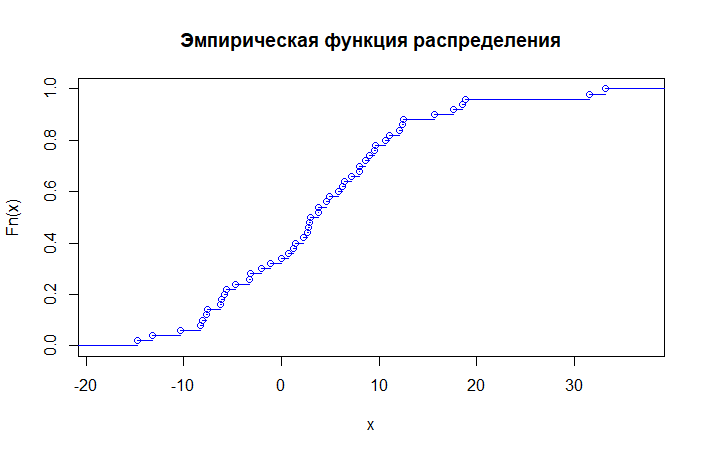
\includegraphics[scale=0.85]{Emp2.png}
	\end{figure}
	\begin{figure}[h!]
		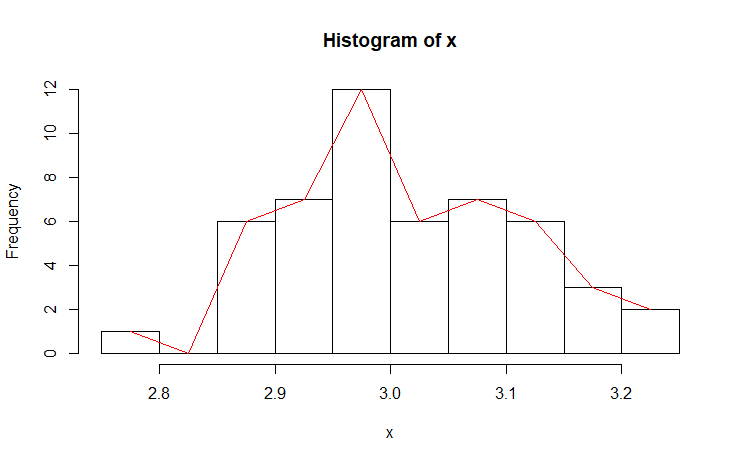
\includegraphics[scale=0.85]{Hist2.png}
	\end{figure}	
\end{proof}

\newpage

\begin{problem}
	Вычислить выборочные аналоги характеристик:
\end{problem}

\begin{proof}
	$ $	
	\begin{enumerate}
		\item Математическое ожидание:
		\begin{equation}	
			\bar x_{\text{в}} = \cfrac1n\sum^{n}_{i=1}(x_i)=3.9774
		\end{equation}
		\item Дисперсия:
		\begin{equation}	
			D_{\text{в}} = \bar{x^2}-\bar{x}^2=\cfrac1n\sum\limits_{i=1}^n(x_i-\bar{x})^2=99.04491
		\end{equation}
		\item Медиана:
		\begin{equation}
			Me = 3.365
		\end{equation}	
		\item Ассиметрия:
		\begin{equation}
			As = \cfrac{\mu_3^*}{\sigma^3} = 0.6413363
		\end{equation}
		\item Эксцесс:
		\begin{equation}
			Ex = \cfrac{\mu_4^*}{\sigma^4}-3 = 0.8044914
		\end{equation}
		\item Вероятность:
		\begin{equation}
			P(x \in [c, d]) = P(x \in [0.00, 14.00]) = F(14.00) - F(0.00) = 0.54 
		\end{equation}
	\end{enumerate}			
\end{proof}


\begin{problem}
	В предположении, что исходные наблюдения являются выборкой из нормального распределения, построить оценку максимального правдоподобия параметров $(a, \sigma^2)$, и соответствующие оценки по методу моментов. Найти смещение оценок. 	
\end{problem}

\begin{proof}
	$ $
	
	Плотность нормального распределения:
	\begin{equation}
		f(x)=\cfrac{1}{\sigma\sqrt{2\pi}} \cdot \exp({-\cfrac{(x-a)^2}{2\sigma^2}})
	\end{equation}

	\begin{enumerate}
		\item Метод максимального правдоподобия

			$L(\vec{x}, a, \sigma^2)=\cfrac{1}{\sigma^n\sqrt{(2\pi)^n}} \cdot \exp({-\cfrac1{2\sigma^2}}\sum\limits_{i=1}^n(x_i-a)^2)$

			$LL(\vec{x}, a, \sigma^2)=\cfrac{n}{2}log2\pi\sigma^2-\cfrac{1}{2\sigma^2}\sum\limits_{i=1}^n(x_i-a)^2$ 	

		$\left\lbrace
		\begin{gathered}
			\cfrac{\partial LL(\vec{x}, a, \sigma^2)}{\partial a}=\cfrac{1}{\sigma^2}\left(\sum\limits_{i=1}^nx_i-na\right)=0 \\
			\cfrac{\partial LL(\vec{x}, a, \sigma^2)}{\partial \sigma^2}=-\cfrac{n}{2\sigma^2}+\cfrac{1}{2(\sigma^2)^2}\sum\limits_{i=1}^n(x_i-a)^2=0 
		\end{gathered}	
		\right.$ \\
		
		$\left\lbrace	
		\begin{gathered}	
			\hat{a}=\cfrac{\sum\limits_{i=1}^nx_i}{n}=\bar{x} \\
			\hat{\sigma^2}=\cfrac1n\sum\limits_{i=1}^n(x_i-\bar{x})^2=S^2 
		\end{gathered}
		\right.$ \\
		
		Найдем значения $\hat{a}=\bar{x}=3.9774$ - выборочное среднее и $\hat{\sigma^2}=S^2=99.04491$ - выборочная дисперсия. \\
		\item Метод моментов
		\begin{align}
			& \text{В случае нормального распределения имеем }a_1'=\mathbb{E}(x)=a \text{ и } a_2'=\mathbb{E}(x^2)=\sigma^2+a^2 
		\end{align}	


			$\tilde{a}=\cfrac{1}{n}\sum\limits_{i=1}^nx_i=\bar{x}=3.9774; \tilde{a^2}+\tilde{\sigma^2}=\cfrac1n\sum\limits_{i=1}^nx_i^2=\bar{x}^2$ 

			$\tilde{a}=\bar{x}=3.9774$
			
			$\tilde{\sigma^2}=\bar{x}^2-\bar{x^2}=\cfrac{(\sum\limits_{i=1}^nx_i^2-\bar{x}\sum\limits_{i=1}^nx_i)}{n}=S^2=99.04491$
			
            Оценки являются несмещенными.
	\end{enumerate}
\end{proof}


\begin{problem}
	Построить доверительные интервалы уровня значимости $\alpha_2$ для параметров $(a, \sigma^2)$ 	
\end{problem}

\begin{proof}
	$ $
	
	$a$:

		$\sqrt{n-1}\left(\cfrac{\bar{x}-n}{s}\right)\sim S_{n-1}$ 
		
		$x_{\alpha}:S_{n-1}(x_{\alpha})=1-\cfrac{\alpha_2}{2}$

	Получаем:
	\begin{equation}
		P\left(-x_{\alpha}\leqslant\sqrt{n-1}\left(\cfrac{\bar{x}-n}{s}\right)\leqslant x_{\alpha}\right)=1-\alpha_2=P\left(\bar{x}-\cfrac{x_{\alpha}s}{\sqrt{n-1}}\leqslant a\leqslant\bar{x}+\cfrac{x_{\alpha}s}{\sqrt{n-1}}\right)
	\end{equation}
	
	ДИ уровня значимости $\alpha_2=0.10$ для $a$:
	\begin{equation}
		[1.638857; 6.315943]
	\end{equation}

	$\sigma^2$: 

		$\cfrac{ns^2}{\sigma^2}\sim \chi^2_{n-1}$ \\


	Выберем $x_{1\alpha}, x_{2\alpha}$ - квантили распределения $\chi^2_{n-1}$ уровня $\cfrac{\alpha_2}2$ и $1-\cfrac{\alpha_2}2$
	
	$p\left(\cfrac{nS^2}{x_{1\alpha}}\leqslant \sigma^2 \leqslant \cfrac{nS^2}{x_{2\alpha}}\right)=1-\alpha_2$ 
	
	ДИ уровня значимости $\alpha_2=0.10$ для $\sigma^2$: 
	\begin{align}
		[74.65098; 145.9534]
	\end{align}
\end{proof}


\begin{problem}
	С использованием теоремы Колмогорова построить критерий значимости проверки простой гипотезы согласия с нормальным распределением с параметрами $a_0, \sigma_0^2$. Проверить гипотезу на уровне значимости $\alpha_2$. Вычислить наибольшее значение уровня значимости, на котором нет оснований отвергнуть данную гипотезу.
\end{problem}

\begin{proof}
	$ $
	
	Простая гипотеза $H_0: a=a_0=-7.00, \sigma^2=\sigma_0^2=10.00$ 
	
	Согласно теореме Колмогорова: \\

	$\sqrt{n}sup|F_n(x)-F_0(x)|\rightarrow K(x)\text{, где $K(x)$ - функция Колмогорова}$ \\

	$K(C_{\alpha_2})=1-\alpha_2=1-0.1=0.9$
	
	$C_{\alpha_2}=C_{0.2}=1.1992$
	
    $H_0: X_1, ..., X_n\sim N(-7.00, 10.00)$ \\
	
	С помощью $R$ вычислим: \\

		$sup|F_n(x)-F_0(x)| = 0.4199428$
		
		$\sqrt{n}sup|F_n(x)-F_0(x)| = 2.969444 > 1.1992$ \\
		
		$\text{Отвергаем гипотезу } H_0$ \\
		
		$p-value = 1.8 \cdot 10^{-14}$ 

	Наибольшее значение уровня значимости, на котором нет оснований отвергнуть гипотезу
\end{proof}


\begin{problem}
	Используя гистограмму частот, построить критерий значимости $\chi^2$ проверки простой гипотезы согласия с нормальным распределением с параметрами $(a_0, \sigma_0^2)$. Проверить гипотезу на уровне значимости $\alpha_2$. Вычислить наибольшее значение уровня значимости, на котором еще нет оснований отвергнуть данную гипотезу. 
\end{problem}

\begin{proof}
	$ $
	
		$H_0: X_1, ..., X_n\sim N(-7.00, 10.00)$ 
		
		$\sum\limits_{i=1}^k\cfrac{(m_i-m_i')^2}{m_i}\rightarrow\chi^2_{\text{кр}}$ 
		
		$\chi^2_{\text{кр}} = \chi^2_4 = 7.77944$ 
	
	Перестроим гистограмму частот, выбрав следующие точки: $(-Inf, -6, 0, 7, 13, Inf)$ 
	\begin{figure}[h]
		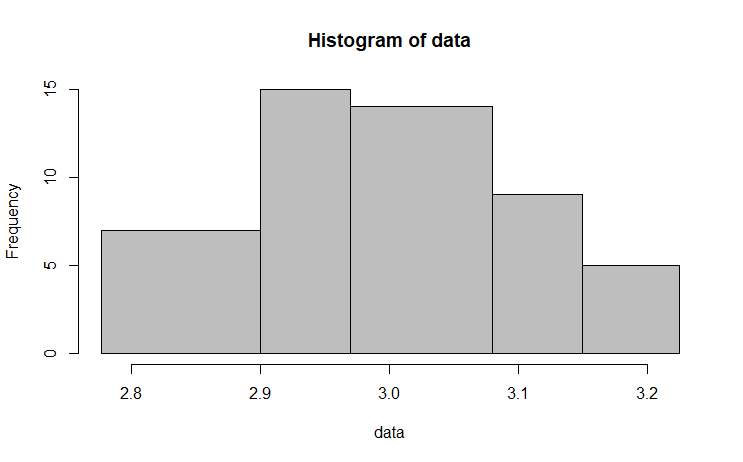
\includegraphics[scale=0.7]{Hist3.png}
	\end{figure} \\
	\begin{tabular}{|c|c|c|c|c|c|c|}
		\hline
		Интервал & $(-\infty; -6]$ & $(-6; 0]$ & $(0; 7]$ & $(7; 13]$ & $(13; \infty)$ & $\sum$ \\ \hline 
		$m_i$ & $7$ & $10$ & $15$ & $12$ & $6$ & $50$ \\ \hline 
		$p_i$ & $0.53982784$ & $0.21820851$ & $0.16120699$ & $0.05800653$ & $0.02275013$ & $1$ \\ \hline 
		$\cfrac{(m_i-m_i^{'})^2}{m_i^{'}}$ & $14.80678546$ & $0.07597088$ & $5.97477145$ & $28.54991124$ & $20.78567469$ & $\chi^2_{\text{набл}}$ \\
		\hline 
	\end{tabular} \\
	
		$\chi^2_{\text{набл}}=70.19311 > \chi^2_{\text{кр}}=7.77944$  \\
		
		$P(\chi^2_{\text{набл}}>70.19311) = 2.065015e-14$ \\
	
	Гипотеза отвергается, наибольшее значение уровня значимости, на котором еще нет оснований отвергнуть гипотезу равно 2.065015e-14.
\end{proof}


\newpage
\begin{problem}
	Построить критерий значимости $\chi^2$ проверки сложной гипотезы согласия с нормальным распределением. Проверить гипотезу на уровне значимости $\alpha_2$. Вычислить наибольшее значение уровня значимости, на котором еще нет оснований отвергнуть данную гипотезу. 
\end{problem}

\begin{proof}
	$ $

		$H_0: X_1, ..., X_n\sim N(a \sigma^2)$ \\
		
		$\sum\limits_{i=1}^k\cfrac{(m_i-np_i(a, \sigma^2))^2}{np_i(a, \sigma^2)}\rightarrow\chi^2_{\text{кр}}$ \\

	Метод минимизации хи-квадрат: \\

	$\underset{a, \sigma^2}{argmin}\sum\limits_{i=1}^k\cfrac{(m_i-np_i(a, \sigma^2))^2}{np_i(a, \sigma^2)}\rightarrow\chi^2_{\text{кр}}$ \\

	Задача реализована в R с помощью скрипта: \\
	
	$\begin{gathered}
		P<-function(a)\{ \hfill \\
        p <- 0 \hfill \\
        p[1] <- pnorm(-6, a[1], a[2]) \hfill \\
        p[2] <- pnorm(0, a[1], a[2]) - sum(p) \hfill \\
        p[3] <- pnorm(7, a[1], a[2]) - sum(p) \hfill \\
        p[4] <- pnorm(13, a[1], a[2]) - sum(p) \hfill \\
        p[5] <- 1 - sum(p) \hfill \\
        p\} \hfill \\
        X2 <- function(a)\{g <- n*P(a); f <- (nu-g)^2/g; sum(f)\} \hfill \\
        nu <- c(7,10,15,12,6) \hfill \\
        a <- c(mean(data), sqrt(var(data))) \hfill \\
        XM <- nlm(X2, a) \hfill \\
	\end{gathered}$	\\

		$\chi^2_{\text{набл}}=0.3942813, a=3.491842, \sigma=8.511311$ \\
		
		$\chi^2_{\text{набл}} < \chi^2_{\text{кр}}=4.60517$
		
	Сложная гипотеза согласия с нормальным распределением принимается.

		$P(x > 0.3942813) = 0.8210752$

	Наибольшее значение уровня значимости, на котором еще нет оснований отвергнуть гипотезу равно 0.8210752
\end{proof}


\begin{problem}
	Построить наиболее мощный критерий проверки простой гипотезы о нормальности с параметром $(a, \sigma^2)=(a_0, \sigma_0^2)$ при альтернативе нормальности с параметром $(a, \sigma^2)=(a_1, \sigma_1^2)$. Проверить гипотезу на уровне значимости $\alpha_2$. Что получится, если поменять местами основную и альтернативную гипотезы?
\end{problem}

\begin{proof}
	$ $
	
	Отношение правдоподобия ($\sigma_0 = \sigma_1$):
	
		$l(x)=\cfrac{L(x, a_1, \sigma_1^2)}{L(x, a_0, \sigma_0^2)}=\cfrac{\sigma_0^n}{\sigma_1^n}\exp\left(\cfrac{1}{2\sigma_0^2}\left(\sum\limits_{i=1}^n(x_i-a_0)^2-\sum\limits_{i=1}^n(x_i-a_1)^2\right)\right)=$
		
		$=\exp\left(\cfrac{1}{2\sigma_0^2}\sum\limits_{i=1}^n-2x_ia_0+a_0^2+2x_ia_1-a_1^2\right)$
	\\
	
	Логарифмируем:
	\begin{equation}
		\exp\left(\cfrac{1}{2\sigma_0^2}\sum\limits_{i=1}^n-2x_ia_0+a_0^2+2x_ia_1-a_1^2\right)>c\rightarrow \cfrac{1}{2\sigma_0^2}\sum\limits_{i=1}^n(a_0^2-a_1^2)+2x_i(a_1-a_0)>log c
	\end{equation}


		$\cfrac{n(a_0^2-a_1^2)}{2\sigma_0^2}+\cfrac{a_1-a_0}{\sigma_0^2}\sum\limits_{i=1}^nx_i>log c$
		
	    $8.25+0.11\sum\limits_{i=1}^nx_i>logc\rightarrow\sum\limits_{i=1}^nx_i>\cfrac{logc-8.25}{0.11}=c^*$ \\

	Тогда критерий примет вид: \\
	
	$\phi(x)=\left\{
	\begin{gathered}
		1, \sum\limits_{i=1}^nx_i<c^* \\
		p, \sum\limits_{i=1}^nx_i=c^* \\
		0, \sum\limits_{i=1}^nx_i>c^*
	\end{gathered}
	\right. \Rightarrow $ 
	$ \phi(x)=\left\{
	\begin{gathered}
		1, \sum\limits_{i=1}^nx_i<-440 \\
		p, \sum\limits_{i=1}^nx_i=-440 \\
		0, \sum\limits_{i=1}^nx_i>-440
	\end{gathered}
	\right.$ \\
	
	$\sum\limits_{i=1}^nx_i=198>-440$, принимается альтернативная гипотеза о нормальности с параметром $(a_1, \sigma_1^2)$. 
	
	Если поменять местами основную и альтернативную гипотезы, то будет принята основная гипотеза о нормальности с параметром $(a_0, \sigma_0^2)$.
\end{proof}


\begin{problem}
	В пунктах (c) - (g) заменить семейство нормальных распределений на двухпараметрическое семейство распределений Лапласа.
\end{problem}

\begin{proof}
	$ $
	
	Плотность распределения Лапласа: 
	\begin{equation}
		f(x)=\cfrac1{\sqrt{2}\sigma}\exp(-\cfrac{\sqrt{2}}{\sigma}|x-a|)
	\end{equation}
\end{proof}


\begin{problem}
	В предположении, что исходные наблюдения являются выборкой из распределения семейства Лапласа, построить оценку максимального правдоподобия параметров $(a, \sigma^2)$, и соответствующие оценки по методу моментов. Найти смещение оценок. 
\end{problem}

\begin{proof}
	$ $
	
	\begin{enumerate}
		\item Метод максимального правдоподобия

			$l(\vec{x}, a, \sigma^2)=\cfrac{1}{\sigma^n2^{n/2}}\exp(-\cfrac{\sqrt{2}}{\sigma}\sum\limits_{i=1}^n|x_i-a|)$ \\
			
			$ll(\vec{x}, a, \sigma^2) = -nlog(\sigma)-\cfrac{n}{2}log(2)-\cfrac{\sqrt{2}}{\sigma\sum\limits_{i=1}^n}|x_i-a| =$ 
			
			$= -nlog(\sigma)-\cfrac{n}{2}log(2)-\cfrac{\sqrt{2}}{\sigma}\sum\limits_{i=1}^k(a-x_{(i)})-\cfrac{\sqrt{2}}{\sigma}\sum\limits_{i=k+1}^n(x_{(i)}-a) =$ \\
			
			$= -nlog(\sigma)-\cfrac{n}{2}log(2)-\cfrac{\sqrt{2}}{\sigma}ka+\cfrac{\sqrt{2}}{\sigma}\sum\limits_{i=1}^kx_{(i)}-\cfrac{\sqrt{2}}{\sigma}\sum\limits_{i=k+1}^nx_{(i)}+\cfrac{\sqrt{2}}{\sigma}(n-k-1)a =$ \\
			
			$= -nlog(\sigma)-\cfrac{n}{2}log(2)+\cfrac{\sqrt{2}}{\sigma}\sum\limits_{i=1}^kx_{(i)}-\cfrac{\sqrt{2}}{\sigma}\sum\limits_{i=k+1}^nx_{(i)}+\cfrac{\sqrt{2}}{\sigma}(n-k-1)a+\cfrac{\sqrt{2}}{\sigma}(n-2k-1)a$ \\

			$\cfrac{\partial ll(\vec{x}, a, \sigma^2)}{\partial a}=\cfrac{\sqrt{2}}{\sigma}(n-2k-1)$ \\
			
			$\cfrac{\sqrt{2}}{\tilde{\sigma}}(n-2k-1)=0; k = \cfrac{n-1}{2} - \text{выборочная медиана}$ \\
			
			$\tilde{a}\in (x_{(\frac{n}{2})}, x_{(\frac{n}{2}+1)})=(x_{(25)}, x_{(26)})=(2.96, 3.77)=3.365$ \\
			
			$\cfrac{\partial ll(\vec{x}, a, \sigma^2)}{\partial \sigma}=-\cfrac{n}{\sigma}+\cfrac{\sqrt{2}}{\sigma^2}\sum\limits_{i=1}^n|x_i-a|$ \\
			
			$-\cfrac{n}{\tilde{\sigma}}+\cfrac{\sqrt{2}}{\tilde{\sigma}^2}\sum\limits_{i=1}^n|x_i-a|=0$ \\
			
			$\tilde{\sigma}=\cfrac{1}{n}\sum\limits_{i=1}^n|x_i-\tilde{a}|$ \\

		Оценка максимального правдоподобия: \\
		\begin{equation}
			(\tilde{a}, \tilde{\sigma}) = (3.365, 58.18333) 
		\end{equation}
		\item Метод моментов

			$\mathbb{E}(x)=a\rightarrow=\hat{a}=\bar{x}=3.9774$ \\
			
			$\mathbb{D}(x)=\cfrac{2}{\frac{2}{\sigma^2}}=\sigma^2\rightarrow\hat{\sigma^2}=s^2=99.04491$ \\
			
			$(\hat{a}, \hat{\sigma^2})=(\tilde{a}, \tilde{\sigma^2})=(3.9774, 99.04491)$

	\end{enumerate}
	\begin{align}
		& \mathbb{E}(\hat{a})=\mathbb{E}(\bar{x})=a\rightarrow\text{несмещенная оценка} \\
		& \mathbb{E}(\hat{\sigma^2})=\mathbb{E}(s^2)=\frac{n-1}{n}\sigma^2\rightarrow\mathbb{E}(\hat{\sigma^2})-\sigma^2=\frac{n-1}{n}\sigma^2-\sigma^2=-\frac{\sigma^2}{n}\rightarrow\text{смещенная оценка}
	\end{align}
\end{proof}


\begin{problem}
	Построить доверительные интервалы уровня значимости $\alpha_2$ для параметров $(a, \sigma^2)$ 	
\end{problem}

\begin{proof}
	$ $
	
	$a$: \\

		$\cfrac{\sum_{i=1}^nx_i-na}{\sqrt{n\sigma^2}}\rightarrow N(0, 1); \cfrac{\sum_{i=1}^nx_i-na}{\sqrt{ns^2}}\rightarrow N(0, 1)$


	Выберем $t_{\gamma}: \phi(t_{\gamma})=1-\cfrac{\alpha_2}2\Rightarrow t_{\gamma}=1.644854$ \\

		$P\left(-t_{\gamma} \leqslant \cfrac{\sqrt{n}(\bar{x}-a)}{s} \leqslant t_{\gamma}\right)=1-\alpha_2=P\left(\bar{x}-\cfrac{t_{\gamma} s}{\sqrt{n}}\leqslant x \leqslant \bar{x}+\cfrac{t_{\gamma} s}{\sqrt{n}}\right)$ \\

	Отсюда асимптотический ДИ:
	\begin{equation}
		[1.662361, 6.292439]
	\end{equation}

	$\sigma^2$:

		$\sqrt{n}(\tilde{\sigma}-\sigma)\sim N(0, \cfrac{\sigma^2}{2})$ \\
	
		$\cfrac{\sqrt{2n}}{\cfrac{\sqrt{2}}{n}\sum_{i=1}^n|x_i-\tilde{a}|}\left(\cfrac{\sqrt{2}}{n}\sum_{i=1}^n|x_i-\tilde{a}|-\sigma\right)\sim N(0, 1)$ \\

	\begin{align}
		& P\left(-t_{\gamma} \leqslant \cfrac{\sqrt{2n}}{\cfrac{\sqrt{2}}{n}\sum_{i=1}^n|x_i-\tilde{a}|}\left(\cfrac{\sqrt{2}}{n}\sum_{i=1}^n|x_i-\tilde{a}|-\sigma\right) \leqslant t_{\gamma}\right) = 1-\alpha_2 = \\
		& = P\left(\cfrac{\sqrt{2}}{n}\sum_{i=1}^n|x_i-\tilde{a}|-\cfrac{t_{\gamma}\sum_{i=1}^n|x_i-\tilde{a}|}{n^{\frac32}} \leqslant \sigma^2 \leqslant \cfrac{\sqrt{2}}{n}\sum_{i=1}^n|x_i-\tilde{a}|+\cfrac{t_{\gamma}\sum_{i=1}^n|x_i-\tilde{a}|}{n^{\frac32}} \right)
	\end{align}

	Вычислим ДИ:
	\begin{equation}
		[81.23379, 157.79624]
	\end{equation}
\end{proof}


\begin{problem}
	С использованием теоремы Колмогорова построить критерий значимости проверки простой гипотезы согласия с распределением из семейства Лапласса с параметрами $a_0, \sigma_0^2$. Проверить гипотезу на уровне значимости $\alpha_2$. Вычислить наибольшее значение уровня значимости, на котором нет оснований отвергнуть данную гипотезу.
\end{problem}

\begin{proof}
	$ $
	
	Простая гипотеза $H_0: a=a_0=-7.00, \sigma^2=\sigma_0^2=10.00$ 
	
	Согласно теореме Колмогорова: \\

		$\sqrt{n}sup|F_n(x)-F_0(x)|\rightarrow K(x)\text{, где $K(x)$ - функция Колмогорова}$ \\

		$K(C_{\alpha_2})=1-\alpha_2=1-0.1=0.9$ 
		
		$C_{\alpha_2}=C_{0.2}=1.1992$
		
		$H_0: X_1, ..., X_n\sim Laplace(-7.00, 10.00)$ \\

	С помощью $R$ вычислим: \\

		$sup|F_n(x)-F_0(x)| = 0.5143445$ 
		
		$\sqrt{n}sup|F_n(x)-F_0(x)| = 3.636965 > 1.1992$ \\
		
		$\text{Отвергаем гипотезу } H_0$ 
		
		$p-value = 1.8 \cdot 10^{-14}$ 

	Наибольшее значение уровня значимости, на котором нет оснований отвергнуть гипотезу
\end{proof}


\begin{problem}
	Используя гистограмму частот, построить критерий значимости $\chi^2$ проверки простой гипотезы согласия с распределением из семейства Лапласса с параметрами $(a_0, \sigma_0^2)$. Проверить гипотезу на уровне значимости $\alpha_2$. Вычислить наибольшее значение уровня значимости, на котором еще нет оснований отвергнуть данную гипотезу. 
\end{problem}

\begin{proof}
	$ $

		$H_0: X_1, ..., X_n\sim Laplace(-7.00, 10.00)$ \\
		
		$\sum\limits_{i=1}^k\cfrac{(m_i-m_i')^2}{m_i}\rightarrow\chi^2_{\text{кр}}$ \\
		
		$\chi^2_{\text{кр}} = \chi^2_4 = 7.77944$ \\

	Перестроим гистограмму частот, выбрав следующие точки: $(-Inf, -6, 0, 7, 13, Inf)$ 
	\begin{figure}[h]
		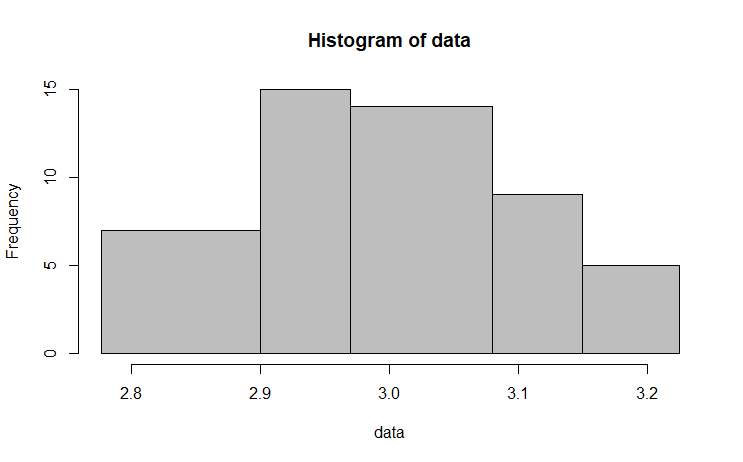
\includegraphics[scale=0.6]{Hist3.png}
	\end{figure} \\
	\begin{tabular}{|c|c|c|c|c|c|c|}
		\hline
		Интервал & $(-\infty; -6]$ & $(-6; 0]$ & $(0; 7]$ & $(7; 13]$ & $(13; \infty)$ & $\sum$ \\ \hline 
		$m_i$ & $7$ & $10$ & $15$ & $12$ & $6$ & $50$ \\ \hline 
		$p_i$ & $0.56593828$ & $0.24826399$ & $0.11675614$ & $0.03948872$ & $0.02955287$ & $1$ \\ \hline 
		$\cfrac{(m_i-m_i^{'})^2}{m_i^{'}}$ & $16.0285515$ & $0.4691403$ & $14.3796781$ & $50.9066573$ & $13.8407570$ & $\chi^2_{\text{набл}}$ \\
		\hline
	\end{tabular}
	\newpage

		$\chi^2_{\text{набл}}=95.62478 > \chi^2_{\text{кр}}=7.77944$ \\
		
		$P(\chi^2_{\text{набл}}>95.62478) \rightarrow 0$ \\

	Гипотеза отвергается, а точность чисел не позволяет вычислить наибольшее значение уровня значимости, на котором еще нет оснований отвергнуть гипотезу (оно крайне близко к 0).
\end{proof}

\begin{problem}
	Построить критерий значимости $\chi^2$ проверки сложной гипотезы согласия с распределением из семейства Лапласса. Проверить гипотезу на уровне значимости $\alpha_2$. Вычислить наибольшее значение уровня значимости, на котором еще нет оснований отвергнуть данную гипотезу. 
\end{problem}

\begin{proof}
	$ $

		$H_0: X_1, ..., X_n\sim Laplace(a \sigma^2)$ \\
		
		$\sum\limits_{i=1}^k\cfrac{(m_i-np_i(a, \sigma^2))^2}{np_i(a, \sigma^2)}\rightarrow\chi^2_{\text{кр}}$ \\

	Метод минимизации хи-квадрат: \\

		$\underset{a, \sigma^2}{argmin}\sum\limits_{i=1}^k\cfrac{(m_i-np_i(a, \sigma^2))^2}{np_i(a, \sigma^2)}\rightarrow\chi^2_{\text{кр}}$ \\



		$\chi^2_{\text{набл}}=2.306802, a=3.908089, \sigma=10.716147$ \\
		
		$\chi^2_{\text{набл}} < \chi^2_{\text{кр}}=4.60517$ \\ 

	Сложная гипотеза согласия с нормальным распределением отвергается.

		$P(x > 2.306802) = 0.3155618$ \\

	Наибольшее значение уровня значимости, на котором нет оснований отвергнуть гипотезу равно $0.3155618$
\end{proof}